% Author: Romulo romuloccomp@gmail.com
% CC: The PGF/TikZ manual

\documentclass{article}

\usepackage{pgf}
\usepackage{tikz}
\usetikzlibrary{arrows,automata}
\usepackage[latin1]{inputenc}
\begin{document}
\begin{figure}
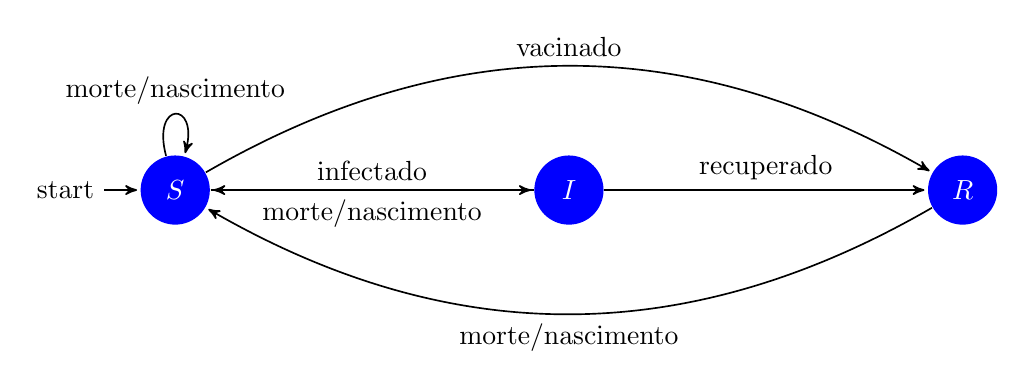
\begin{tikzpicture}[->,>=stealth',shorten >=1pt,auto,node distance=5cm,
                    semithick]
  \tikzstyle{every state}=[fill=blue,draw=none,text=white]

  \node[initial,state] (S)               {$S$};
  \node[state]         (I) [right of=S]  {$I$};
  \node[state]         (R) [right of=I]  {$R$};

  \path (S) edge [loop above] node {morte/nascimento} (S)
            edge [bend left]  node {vacinado} (R)
            edge              node {infectado} (I)            
            
        (I) edge              node {recuperado} (R)
        (I) edge              node {morte/nascimento} (S)
        
        (R) edge [bend left]  node {morte/nascimento} (S);

\end{tikzpicture}
\caption{A caption.}
\end{figure}
\end{document}
